% ICASSP working draft. Quantitative claims are restricted to the sealed H9
% terminal evaluation documented in experiments/h9_paired_counterfactual/.
\documentclass{article}
\usepackage{template/ICASSP2026/spconf}

\usepackage{cite}
\usepackage{booktabs}
\usepackage{amsmath}
\usepackage{graphicx}
\usepackage{url}

\title{SAME-ITEM PAIR RANKING FOR CROSS-CORPUS SPEECH DEEPFAKE DETECTION}

\name{Kirill Borodin$^{1,2}$}
\address{$^{1}$\;lab260, Moscow, Russia\\
$^{2}$\;BitmanagerAI, Dubai, UAE}

\begin{document}
\maketitle

\begin{abstract}
Pairwise objectives are used in speech anti-spoofing, but it is unclear whether
matching a documented natural--synthetic source item, rather than an arbitrary
opposite-class item, improves transfer. We test this question with a controlled
three-way comparison. A compact, fresh-initialized Res2TCNGuard detector is
trained on a shared ODSS source pool using (i) binary cross-entropy (B1), (ii)
the same loss plus random opposite-class ranking (B2), or (iii) same-item
natural--synthetic ranking (P). Source-only selection fixes all hyperparameters,
checkpoints, and the four-seed ensemble before two fixed external evaluations.
P obtains 47.07\%/42.98\%/45.02\% equal error rate (EER) on
SONAR/ArAD/macro, versus 58.88\%/44.69\%/51.78\% for B1 and
56.09\%/47.93\%/52.01\% for B2. Paired trial-bootstrap intervals,
conditional on the frozen ensemble, are P--B1 $[-8.25,-5.25]$ and P--B2
$[-8.54,-5.30]$ percentage points. Thus, under this protocol, same-item
ranking lowers the predeclared two-target macro EER beyond an equal-edge
random-pair control. The documented key is not a transcript-level semantic
annotation; we make no state-of-the-art or causal representation claim.
\end{abstract}

\begin{keywords}
speech deepfake detection, anti-spoofing, pairwise ranking, cross-corpus
generalization, controlled evaluation
\end{keywords}

\section{Introduction}
\label{sec:intro}

Speech anti-spoofing can fail when a detector is moved to a new corpus or
generator family. Such shifts are often differences in data distribution,
rather than simply a harder instance of the original task~\cite{muller2024harder}.
Pairwise learning is one route to improve a representation: a Siamese
anti-spoofing system learns class agreement between two samples~\cite{xie2021siamese},
supervised contrastive learning has been combined with cross-entropy for spoof
detection~\cite{tran2024contrastive}, and bonafide-pair learning aligns two
augmentations of a bonafide utterance~\cite{kim2025bpl}. We do not claim
pairwise supervision as new. Instead, we ask whether a documented same-item
pairing changes transfer relative to a fixed, equal-edge random-pair control.

We test this with naturally paired resynthesis data. ODSS provides documented
natural and synthetic variants of source utterances~\cite{yaroshchuk2023odss}.
We compare same-item ranking to two controls that preserve the source
pool, network, binary objective, number of ranking edges, rank weight,
optimizer, and selection procedure. The random-pair control is important:
without it, a gain could be attributed to any added margin term rather than the
documented same-item relation.

Our contributions are:
\begin{itemize}
  \item a same-item paired-ranking objective and an equal-edge,
  stratum-matched random-ranking control for separating the documented pairing
  key from generic rank regularization;
  \item a source-only training/selection protocol with fresh initialization,
  voice-disjoint source development, target-label firewall, and source--target
  waveform-fingerprint audit; and
  \item a two-target, four-seed terminal evaluation in which same-item ranking
  lowers EER relative to both controls under a precommitted,
  ensemble-conditional trial-bootstrap gate.
\end{itemize}

\section{Controlled same-item ranking}
\label{sec:method}

\subsection{Matched source pool}

We use ODSS revision \texttt{1968e6d0} as the only training source. Its
metadata yields 7,961 complete groups, each containing one natural recording,
a VITS resynthesis, and a FastPitch/HiFiGAN resynthesis. Groups are keyed by
corpus, speaker, and stem. We retain 23,883 trials (7,961 bona fide and
15,922 spoof) and remove 3,071 unmatched VITS rows from \emph{all} methods.
Thus BCE does not receive additional unpaired data. A deterministic
language-stratified split assigns each source voice key to either train or
source development.

Let $z(x)$ be a spoof-evidence logit and $(x_s,x_b)$ a spoof--bona-fide edge.
Every method receives the same class-balanced BCE batches. B1 minimizes
$\mathcal{L}_{\mathrm{BCE}}$. For $m\in\{\mathrm{B2},\mathrm{P}\}$, the
objective is
\begin{equation}
\begin{aligned}
\mathcal{L}_{m} &= \mathcal{L}_{\mathrm{BCE}} \\
                 &\quad + \lambda\mathcal{L}_{\mathrm{rank}},
\end{aligned}
\label{eq:total}
\end{equation}
where
\begin{equation}
\mathcal{L}_{\mathrm{rank}}=
\frac{1}{|E|}\sum_{(x_s,x_b)\in E}
\max\{0,1-[z(x_s)-z(x_b)]\}.
\label{eq:rank}
\end{equation}

\begin{figure*}[!t]
  \centering
  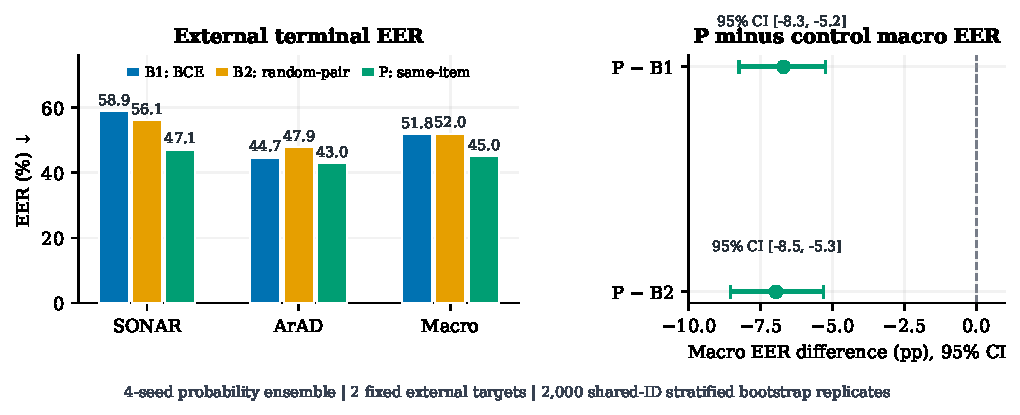
\includegraphics[width=\textwidth]{figures/fig_h9_pcr_terminal_eer.pdf}
  \caption{Sealed terminal evaluation. \textbf{Left:} EER of the four-seed
  probability ensemble on the two fixed external targets and their unweighted
  macro average (lower is better). \textbf{Right:} fixed 95\% percentile
  intervals from 2,000 shared-ID, label-stratified bootstrap resamples of
  macro-EER differences, conditional on the frozen four-seed ensemble. The
  figure is display-only: it reads hash-pinned
  terminal metrics, decision, bootstrap, and provenance but no raw prediction
  or label table.}
  \label{fig:terminal}
\end{figure*}

P uses the 15,922 natural--synthetic edges from the same documented group. B2
uses exactly the same spoof endpoints and edge count, but pairs each with a
different-group bona-fide trial selected deterministically within its
split/language/source-corpus/generator stratum. Thus the intended B2--P
difference is same-item versus different-item pairing. The key is metadata,
not a transcript or semantic-equivalence proof; it can bundle speaker,
recording, duration, and phonetic correspondence with the documented item.

\subsection{Frozen optimization and terminal firewall}

All models are freshly initialized instances of the public 172k-parameter
Res2TCNGuard architecture~\cite{borodin2024res2tcn}; its released
ASVspoof-pretrained checkpoint is prohibited. We use BF16 autocast, batch 24,
AdamW ($10^{-4}$ learning rate, $10^{-2}$ weight decay), no augmentation, and
at most six epochs. A source-only grid over rank weight $\{0.1,0.3,1.0\}$
selects $1.0$ by mean voice-disjoint development EER; that P-selected value is
imposed unchanged on B2. Four fixed seeds use the lowest-development-EER
checkpoint (lower epoch on a tie). No target audio, label, metric, or score
selects a source choice.

The terminal targets are fixed SONAR (3,948 trials) and ArAD (3,570 trials)
releases from the Speech DF Arena ecosystem~\cite{dowerah2026arena}. After all
12 source checkpoints are hash-sealed, we materialize label-free target records
and separately hash labels. The evaluator verifies every audio byte hash and
canonical 16-kHz waveform fingerprint, writes all raw predictions, then opens
labels once. It rejects any exact source--target fingerprint collision; none is
observed. We report EER (the threshold at which false-accept and false-reject
rates are equal; lower is better) and AUROC with spoof as the positive class
from the mean spoof probability of the four frozen seeds. Target metrics never
enter model selection; we nevertheless do not call this evaluation blind because
historical target rows for the excluded public checkpoint were visible during
the architecture-provenance audit.

\section{Results}
\label{sec:results}

\subsection{Source-only selection}

The rank weight is the only loss hyperparameter selected from source
development. Before any target materialization, we run the fixed P grid with
four seeds per value and choose lower mean development EER (lower weight on a
tie). Table~\ref{tab:lambda} shows the complete selection evidence. The chosen
$\lambda=1.0$ is then imposed on B2 as well as P, so a terminal difference
cannot be caused by a different ranking scale. B2 is deliberately not tuned at
its own optimum: it is the fixed P-lambda, equal-edge control. All methods
share four fresh initializations, BF16 batch 24, four workers, and at most six
epochs; B1 does not execute rank-edge forwards, so this is a matched training
envelope rather than equal wall-clock compute across all three methods.

\begin{table}[t]
  \caption{Complete source-only P rank-weight selection. Mean development EER
  is over four fixed seeds; lower is better. The selected value is reused
  unchanged for B2 and P terminal fits.}
  \label{tab:lambda}
  \centering
  \footnotesize
  \begin{tabular}{lrrr}
    \toprule
    $\lambda$ & 0.1 & 0.3 & 1.0 \\
    \midrule
    Mean dev. EER (\%) & 33.60 & 25.92 & \textbf{22.05} \\
    \bottomrule
  \end{tabular}
\end{table}

\subsection{Terminal external evaluation}

Figure~\ref{fig:terminal} reports the complete predeclared primary EER
comparison. P has lower ensemble EER than B1 and B2 on both targets. Its
45.02\% macro EER is 13.05\% relatively lower than B1 (51.78\%) and 13.44\%
relatively lower than B2 (52.01\%). The predefined 2,000-replicate,
label-stratified shared-ID trial bootstrap (seed 2909), conditional on the
frozen four-seed ensemble, gives P--B1 $-6.70$ pp (95\% CI $[-8.25,-5.25]$)
and P--B2 $-6.97$ pp (95\% CI $[-8.54,-5.30]$). Both intervals are below zero,
and all precommitted terminal checks pass.

Table~\ref{tab:diagnostics} gives score diagnostics and class counts. P has
the highest AUROC on both targets, but all values and the weak absolute EERs
must be read as a narrow transfer comparison rather than a deployment result.

\begin{table}[t]
  \caption{Terminal score diagnostics. Scores are mean spoof probabilities;
  AUROC treats spoof as positive. Target counts are bona-fide/spoof.}
  \label{tab:diagnostics}
  \centering
  \footnotesize
  \begin{tabular}{llrr}
    \toprule
    Target (bona/spoof) & Method & EER (\%) & AUROC \\
    \midrule
    SONAR (2274/1674) & B1 & 58.88 & .411 \\
                      & B2 & 56.09 & .428 \\
                      & P  & \textbf{47.07} & \textbf{.557} \\
    \midrule
    ArAD (484/3086) & B1 & 44.69 & .586 \\
                    & B2 & 47.93 & .519 \\
                    & P  & \textbf{42.98} & \textbf{.615} \\
    \bottomrule
  \end{tabular}
\end{table}

\begin{table}[t]
  \caption{Per-seed macro EER (\%). Each value averages SONAR and ArAD for
  one frozen seed; the predeclared probability ensemble in Fig.~\ref{fig:terminal}
  is the primary endpoint.}
  \label{tab:seeds}
  \centering
  \footnotesize
  \begin{tabular}{lrrrr}
    \toprule
    Method & 9101 & 9102 & 9103 & 9104 \\
    \midrule
    B1 & 50.00 & 50.59 & 53.78 & 46.26 \\
    B2 & 53.05 & 50.67 & 54.47 & 47.58 \\
    P  & 53.30 & 49.26 & 45.92 & 41.10 \\
    \bottomrule
  \end{tabular}
\end{table}

The result should not be confused with a strong absolute detector. P remains
at 47.07\% EER on SONAR and 42.98\% on ArAD. Further, the decision concerns a
predeclared four-seed ensemble: individual-seed macro EER varies from 41.10\%
to 53.30\% for P. The trial-bootstrap intervals do not resample source voices,
training seeds, or a new random-pair draw. We therefore interpret the result
as controlled evidence that documented same-item pairing matters beyond the
random-pair margin in this protocol, rather than evidence that linguistic
content has been causally removed from a representation.

\section{Protocol checks and scope}
\label{sec:scope}

The comparison has four deliberate safeguards. First, B1, B2, and P share the
complete matched-only source pool, so P is not given extra examples or an
easier class mix. Second, B2 reuses every P spoof endpoint, the rank-edge
count, the selected $\lambda$, and the split/language/source/generator
marginals; it changes the bona-fide partner from same-group to different-group.
Third, the public checkpoint is excluded and each result is
from a fresh initialization, avoiding undeclared pretraining. Fourth, the
source checkpoint ledger is complete before either target is materialized;
target records omit labels until all raw predictions are emitted. The evaluator
also byte-verifies every copied target payload and rejects exact canonical
source--target waveform duplicates. These checks do not prove that source and
target have no speaker, text, or generator lineage in common, but they rule out
the defined direct-content and selection failures.

The result is not a generic claim for pairwise learning. B2 is sometimes worse
than BCE (52.01\% versus 51.78\% macro EER), so the observed gain is not
explained by adding Eq.~\eqref{eq:rank} alone. Nor is it a claim that P is the
best anti-spoofing model: the absolute EERs remain high. The appropriate
interpretation is a controlled interaction in one source/architecture/target
configuration: documented natural--synthetic pairing provides useful
supervision beyond a random opposite-class partner under the fixed protocol.

For reproducibility, the public lab260ru GitHub organization hosts repository
``icassp\_antispoofing'' at immutable tag ``h9pcr-d1.'' It contains the source
code, frozen protocol, compact ledgers, and result note under the paired-
counterfactual experiment directory. The release records source pairing/
exclusion and selection ledgers, checkpoint hashes, separate target record/
label manifests, raw-prediction hash, metrics, seed metrics, bootstrap draws,
and a decision record; source and target audio remain under their original
dataset licenses. The figure reads only four hash-pinned compact terminal
artifacts. These materials make the result auditable but do not turn the
completed targets into a tuning set for a future extension.

\section{Discussion and limitations}
\label{sec:discussion}

The B2 result is informative: adding a rank loss alone does not reproduce P,
despite its matched edge count and strata. This pattern is consistent with the
value of pairing natural and synthetic versions of the documented source item.
However, the filename-derived content key is not a transcript-level proof of
semantic equivalence, and the experiment does not measure which representation
attribute changes. It uses one compact architecture, one source dataset, two
fixed targets, and a four-seed ensemble. The weak absolute EER and seed
heterogeneity limit deployment claims. A new target or architecture replication
must be independently predeclared; it cannot tune the completed protocol.

\section{Conclusion}

Same-item pair ranking lowers the locked two-target transfer EER of a fresh
compact anti-spoofing detector relative to both same-pool BCE and an equal-edge
random-pair ranking control. The result is supported by a source-only selection
chain, target-label firewall, zero exact waveform collisions, and
ensemble-conditional paired trial-bootstrap intervals. It motivates further
independently frozen replications, not a claim of universal robustness or a
causal linguistic-content mechanism.

\clearpage
\bibliographystyle{template/ICASSP2026/IEEEbib}
\bibliography{references}

\end{document}
